%Chapter 5

\renewcommand{\thechapter}{5}

\chapter{Quasi-integrable Octupole Lattice}

As introduced in Chapter 1, a quasi-integrable octupole lattice is proposed as a way to mitigate space charge in accelerator rings. Large amplitude-dependent tune spreads, driven by strong nonlinear magnet inserts, lead to decoupling from incoherent tune resonances. This reduces intensity-driven beam loss while quasi-integrability ensures a well-contained beam. In this chapter I discuss on-going work to install and interrogate a long-octupole channel at the University of Maryland Electron Ring (UMER), as well as explore simulated properties of the proposed nonlinear lattice. This is a discrete insert that occupies 20 degrees of the ring, consisting of independently powered printed circuit octupole magnets. Transverse confinement is obtained with quadrupoles external to this insert. Operating UMER as a non-FODO lattice, in order to meet the beam-envelope requirements of the quasi-integrable lattice, is a challenge. 




\section{Toy Model}

The prescription for a strongly nonlinear lattice with 1 or 2 analytic invariants is laid out in Danilov and Nagatisev's 2010 publication [\cite{Danilov2010}].


\begin{figure}
\centering
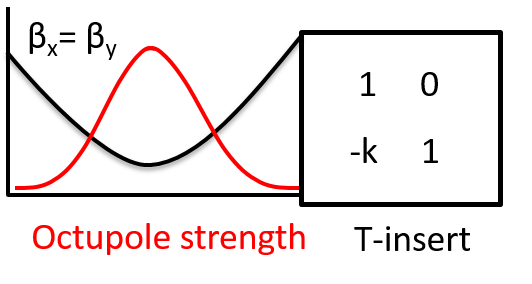
\includegraphics[width=.3\textwidth]{2.figures/toy_model.png}
\caption{Simple quasi-integrable system: FOFO focusing with nonlinear insert }
\label{fig:toymodel}
\end{figure}




\subsection{Frequency Map Analysis of Chaotic Octupole Lattice}

%todo: Cover WARP and Elegant models, estimate tune prediction


\subsection{Steering Tolerances}

The effect of background fields on the low-rigidity UMER beam is significant. The closed orbit is necessarily not straight but arcs between corrector magnets. The vertical field is almost constant at all ring sections at an average of 400 mG for approximately 2.2° of bend angle per horizontal dipole. The radial field has a sinusoidal variation with amplitude 200 mG, for maximum bend angle of 2.2° per vertical corrector. The effect on particle stability must be considered for the strongly nonlinear lattice. 

A simulation model in the WARP PIC code of a 64 cm octupole channel with an ideal linear thin-lens transformation was used to probe dynamic aperture and tune spread under these non-ideal conditions. In the simulation, a constant closed orbit distortion term is included in the trajectory calculations for each particle as thin lens transformations.

We see that the presence of a vertical background field, there is an $80\%$ loss of dynamic aperture at 400 mG when compared to the ideal case. The addition of radial field causes severe loss of stability. We choose to place the nonlinear channel at a azimuthal location of locally low radial field. Additionally, shielding the background field down to 100 mG or less will limit dynamic aperture loss to $92\%$ of ideal area. Dynamic aperture calculations assume a round beam through the channel.

\subsection{Sensitivity to external focusing}
% Beta and tune errors

\subsection{Space Charge in octupole lattice}
% Early halo evolution studies.

\cite{Webb2013}, \cite{WebbIPAC2013} %%todo: cite Radiasoft 2017 IOTA meeting presentation?

\section{Matching UMER for nonlinear experiments}


\section{Full ring simulation of octupole lattice}

